% REV: Revised manuscript after MDPI reviews; comments marked with % REV indicate modified or newly added sections.
%  LaTeX support: latex@mdpi.com

\documentclass[applsci,article,submit,pdftex,moreauthors]{Definitions/mdpi}

\usepackage{xr}
\usepackage{booktabs}
\usepackage{amssymb}   % dla \checkmark
\usepackage{fontawesome5}
\usetikzlibrary{positioning}
\usepackage{xcolor}
\usepackage{soul}
\sethlcolor{yellow}

\newcommand{\rev}[1]{\hl{#1}}
\soulregister\cite7
\soulregister\citep7
\soulregister\citet7
\soulregister\ref7
\soulregister\eqref7
\soulregister\url7
\soulregister\texttt7
\soulregister\textbf7
\soulregister\emph7

\IfFileExists{supplement_mdpi.aux}{\externaldocument{supplement_mdpi}}{}

\setlength{\headheight}{20pt}
\addtolength{\topmargin}{-7pt}

\firstpage{1}
\makeatletter
\setcounter{page}{\@firstpage}
\makeatother
\pubvolume{1}
\issuenum{1}
\articlenumber{0}
\pubyear{2026}
\copyrightyear{2026}
\datereceived{ }
\daterevised{ }
\dateaccepted{ }
\datepublished{ }

\Title{PU-Based Quality Classifier for LLM Training Texts}

\newcommand{\orcidauthorA}{0000-0001-7408-6060}
\newcommand{\orcidauthorB}{0000-0002-7683-4787}

\Author{Kacper Paczutkowski \textsuperscript{1}\orcidA{} and Konrad Furma\'{n}czyk \textsuperscript{1}\orcidB{}}
\AuthorNames{Kacper Paczutkowski and Konrad Furma\'{n}czyk}
\address{%
\textsuperscript{1} \quad Institute of Information Technology, Warsaw University of Life Sciences, Warsaw, Poland; kacper\_paczutkowski@sggw.edu.pl; konrad\_furmanczyk@sggw.edu.pl}
\corres{Correspondence: kacper\_paczutkowski@sggw.edu.pl}

% REV: Abstract updated with quantitative results and explicit gains over Naive, per Reviewer 2.
\abstract{We study positive-unlabeled (PU) learning for classifying Polish texts intended for large-language-model training. The paper presents a Python reimplementation of the training and evaluation pipeline from earlier work, together with preprocessing tailored to the SpeakLeash corpora used in our experiments. We evaluate six PU methods: naive, clust, strict-lassclust, non-strict-lassclust, lassojoint, and spy under both classic and MVC non-SCAR labelling schemes. Across the benchmark, the best F1 reaches 0.906 on open subtitles corpus under classic labelling and 0.900 under MVC labelling; the largest absolute gain over the Naive baseline is 0.811 F1 points on ulotki medyczne and 0.758 on plwiki in the classic setting. The experimental workflow supports multiple labelling rates c calc and repeated random seeds, and evaluates models with AUC, PR-AUC, and F1 as the main metrics. Our study focuses on six SpeakLeash datasets spanning different domains: plwiki, open subtitles corpus, job offers corpus, ISAP corpus, ulotki medyczne, and wolne lektury corpus. For each dataset, we construct a binary PU setup from the quality field, where HIGH is treated as positive and LOW is negative, while other values are removed. The resulting preprocessed tables retain only the selected linguistic and structural features, rescale numeric variables to the $[0,1]$ range, and remove the raw text column.}

% REV: Keywords updated (Bielik.AI removed, data cleaning added) per Reviewer 2.
\keyword{positive-unlabeled learning; text quality; Polish texts; SpeakLeash; natural language processing; data cleaning}

\begin{document}

% REV: Introduction expanded with clearer motivation and modern references (FineWeb, GneissWeb, CQF, Romanian LLM filtering, ScalePU) per Reviewers 1--2.
\section{Introduction}

Positive-unlabeled learning is a natural fit for text quality assessment when only a subset of high-quality examples is explicitly identified and the remaining documents are partially observed. This scenario arises naturally whenever collecting negative labels is costly or semantically ambiguous -- a situation that directly characterizes large-scale text corpora such as those studied here~\cite{bekker2020survey}.

The theoretical foundations of PU learning have been well-established. Bekker and Davis~\cite{bekker2020survey} provide a comprehensive survey covering label-frequency estimation, class-prior estimation, and algorithm design under partial supervision. Liu et al.~\cite{liu2002spy} formalized this structure for text classification and introduced the Spy technique, in which a fraction of labeled positives is temporarily moved into the unlabeled set to calibrate a threshold for reliable negative extraction. Nigam et al.~\cite{nigam2000em} showed that even a small labeled set combined with unlabeled documents via Expectation-Maximization substantially reduces classification error -- an early demonstration that the unlabeled majority carries exploitable signal. \rev{The PU framework has since been applied across diverse domains: Fusilier et al.~\cite{fusilier2015opinionspam} showed that a PU classifier trained solely on confirmed fake hotel reviews achieves F-measure on par with fully supervised baselines, and Furma\'{n}czyk et al.~\cite{pu_classic_propensity,mdai25_mvc} developed propensity-based and cluster-assisted logistic methods that form the direct methodological basis of the present work.} \rev{Recent work has extended PU learning to settings with extremely few labeled positive examples.} \rev{Dai et al.~\cite{dai2026scalepu} derived theoretical conditions under which reliable learning remains possible and proposed the ScalePU framework for such highly label-scarce scenarios.} \rev{A complementary line of research concerns class-prior estimation under distribution shift.} \rev{Mielniczuk et al.~\cite{mielniczuk2026priorshift} proposed a kernel-embedding estimator for PU data that explicitly accounts for prior shift and established non-asymptotic theoretical guarantees for the estimator.} \rev{More recently, Liu et al.~\cite{liu2026puicl}  proposed PUICL, an in-context learning framework based on pretrained transformers that performs PU classification without task-specific fine-tuning.} \rev{These recent developments demonstrate the rapid expansion of PU learning toward both stronger theoretical guarantees and modern foundation-model architectures.} \rev{However, they have not yet been systematically evaluated for stylometric quality assessment of Polish LLM training corpora.} \rev{Mansouri et al.~\cite{mansouri2026activepu} provide the first theoretical analysis of the label complexity of active PU learning, studying how an adaptive querying strategy can reduce the number of labels needed to recover a reliable classifier.}

A critical practical consideration is that the labeling mechanism in quality-annotation pipelines is unlikely to satisfy the \emph{Selected Completely At Random} (SCAR) assumption. Formally, SCAR requires $e(\mathbf{x}) := P(S=1 \mid Y=1, \mathbf{x}) = c$ for some constant $c$ independent of $\mathbf{x}$ -- that is, every positive instance is equally likely to be labeled regardless of its features. In practice, however, annotators preferentially label visually prominent documents -- those with higher lexical density or greater length -- making the labeling probability feature-dependent and thus violating the SCAR assumption~\cite{bekker2020survey}. This non-SCAR regime motivates the use of propensity-based labeling schemes that explicitly model $e(\mathbf{x})$~\cite{pu_classic_propensity}.
From this perspective, document-quality annotation for LLM training texts can be viewed as a PU learning problem under a non-SCAR labeling mechanism: only a subset of truly high-quality documents receives an explicit positive label, while the remaining pool is left unlabeled and therefore contains a mixture of high- and low-quality texts. The probability that a high-quality document is annotated as such then depends on its observable attributes $\mathbf{x}$ (for example length, lexical density, or domain), which matches the instance-dependent propensity setting $e(\mathbf{x}) = P(S=1 \mid Y=1, \mathbf{x})$ emphasized in recent PU learning work~\cite{bekker2020survey}.

\rev{The practical stakes of quality filtering in Polish NLP are illustrated by the SpeakLeash-based Bielik model family~\cite{bielik7b,bielik11bv3,ociepa2026bielikv3tok}: successive versions (7B~v0.1, 11B~v2, 11B~v3) were trained on best quality SpeakLeash corpora and demonstrated that curated Polish data is essential for competitive downstream performance.} Penedo et al.~\cite{penedo2024fineweb} reached a structurally identical conclusion for English web text: their FineWeb-Edu classifier -- trained on a small LLM-annotated positive seed and a large unlabeled CommonCrawl pool -- is, in effect, a PU learner, even though it is not explicitly framed as such. \rev{More recently, Emami~Gohari et al.~\cite{emami2026gneissweb} demonstrated at scale that combining heuristic and classifier-based quality signals into a unified pipeline (GneissWeb) substantially improves LLM pretraining outcomes, reinforcing the importance of principled data-quality filtering for both English and multilingual corpora.} \rev{Negoi\'{t}a et al.~\cite{negoita2026romanianllm} show that diversity-aware quality filtering strongly benefits Romanian LLM pretraining, highlighting the relevance of classifier-based filters for under-resourced languages beyond Polish.} Li et al.~\cite{li2024scalingfilter} caution, however, that quality filters anchored to a fixed high-quality reference set introduce selection bias and reduce corpus diversity, because the filtering criterion is implicitly shaped by the characteristics of the seed collection rather than by the downstream task. \rev{Nait Saada et al.~\cite{saada2026cqf} further argue that classifier-based quality scores can conflate changes in corpus composition with genuine quality improvements, challenging the view that classifier-based quality filtering (CQF) always captures an intrinsic notion of data quality.} \rev{Langlais et al.~\cite{langlais2026commoncorpus} address the data availability problem from a different angle, releasing Common Corpus -- the largest open and fully licensed collection for multilingual LLM pretraining -- which covers Polish among dozens of European languages and establishes a reproducible baseline for open-science LLM research.}

This observation reinforces the need for principled PU methods that explicitly model the labeling propensity $e(\mathbf{x})$ and decouple it from the classification objective -- exactly the distinction drawn by the non-SCAR framework evaluated in the present work. In this paper we study whether dedicated PU methods can classify Polish texts in a reproducible way across heterogeneous domains and data sizes. The full experimental pipeline is implemented in Python\footnote{Selected classification scripts were rewritten by the authors from their earlier R implementations (\url{https://github.com/kapacc/mdai25-clusters-scripts}) into Python with assistance from GitHub Copilot, mainly using a GPT-Codex model. The current codebase is available at \url{https://github.com/kapacc/pullm}.} and separates labelling, preprocessing, and model training into distinct stages.

% REV: New subsection for literature survey and explicit contributions, per Reviewers 1--3.
\subsection{Related Work and Contributions}

\rev{Modern data filtering for LLM training increasingly uses classifier-guided pipelines such as FineWeb-Edu~\cite{penedo2024fineweb}, the GneissWeb framework~\cite{emami2026gneissweb}, and scaling-aware quality filters such as ScalingFilter~\cite{li2024scalingfilter}.} \rev{Those approaches motivate our study, but they still do not answer the PU-specific question of how to model positive-only labeling under non-SCAR conditions for Polish corpora.} \rev{Recent work on low-resource languages demonstrates that similar classifier-based quality filtering pipelines can substantially improve pretraining data for Romanian~\cite{negoita2026romanianllm}.} \rev{At the same time, Nait Saada et al.~\cite{saada2026cqf} provide a critical analysis of CQF-style filters for LLM pretraining, showing that classifier scores may not always correspond to intrinsic data quality; we acknowledge this as a limitation of classifier-based filters and treat our PU classifiers primarily as tools for prioritizing data rather than as complete quality metrics.} \rev{Langlais et al.~\cite{langlais2026commoncorpus} complement this picture by providing a large-scale multilingual resource with explicit provenance metadata, enabling future work to benchmark quality classifiers under reproducible and ethically vetted conditions.} \rev{On the PU learning side, Wang et al.~\cite{wang2026pubenchmark} recently proposed a standardized evaluation framework for PU algorithms that highlights the importance of realistic experimental conditions and reproducible benchmarking -- a concern shared by the present work.} \rev{Dai et al.~\cite{dai2026scalepu} complement this perspective with a theoretical analysis of PU learning under extreme label scarcity and a variance-regularized ScalePU estimator.} \rev{Mielniczuk et al.~\cite{mielniczuk2026priorshift} address the related problem of class-prior estimation when the target distribution shifts, which is directly relevant to our cross-domain evaluation setting.} \rev{The PUICL model of Liu et al.~\cite{liu2026puicl} demonstrates that in-context learning can be applied to PU classification without dataset-specific training, a direction that could further reduce the annotation overhead in future extensions of this work.} \rev{Mansouri et al.~\cite{mansouri2026activepu} provide formal guarantees on the label complexity achievable by an adaptive querying strategy in the PU setting, motivating future work on active annotation for SpeakLeash corpora.}

\rev{The concrete contributions of this paper are:}
\begin{itemize}
\item \rev{First comprehensive benchmark of PU-learning methods for Polish LLM training corpora.}
\item \rev{Evaluation under two different non-SCAR labeling mechanisms.}
\item \rev{Cross-domain study across six heterogeneous SpeakLeash datasets.}
\item \rev{Practical recommendations for PU-learning deployment in LLM data filtering.}
\item \rev{Open-source Python implementation enabling reproducible research.}
\end{itemize}

% REV: Novelty table added to clarify substantive innovations vs earlier work, per Reviewers 1 and 3.
\rev{Table~\ref{tab:novelty_comparison} summarizes the substantive differences between the previous our non-SCAR study and the present manuscript.}

\begin{table}[t]
\centering
\caption{Substantive novelty of the present manuscript relative to the our earlier non-SCAR study.}
\label{tab:novelty_comparison}
\small
\begin{tabularx}{\textwidth}{l>{\raggedright\arraybackslash}X>{\raggedright\arraybackslash}X}
\toprule
\textbf{Aspect} & \textbf{Earlier work} & \textbf{Present manuscript} \\
\midrule
Scope & One PU benchmarking setup centered on clustering and logistic modeling under non-SCAR assumptions & Six PU methods compared under two non-SCAR label-generation schemes across six SpeakLeash corpora \\
Data handling & Earlier pipeline and narrower experimental scope & Reimplemented in Python with shared preprocessing, repeated seeds, and unified evaluation protocol \\
Method coverage & Cluster-assisted and logistic non-SCAR variants & Adds Naive, Strict-LassClust, Non-Strict-LassClust, LassoJoint, and Spy as direct comparators \\
Interpretation & Method comparison focused on algorithmic behavior & Adds dataset-level discussion, limitations, and practical method-selection guidance for LLM filtering \\
Reporting & Earlier benchmark summary & Expanded tables, stability analysis, runtime summaries, and reviewer-oriented interpretation \\
\bottomrule
\end{tabularx}
\end{table}

\begin{table}[H]
\caption{Comparison of selected related work and the present study.}
\label{tab:novelty}
\centering
\begin{tabular}{lllll}
\toprule
\textbf{Work} &
\textbf{Application Domain} &
\textbf{PU Learning} &
\textbf{Non-SCAR} &
\textbf{LLM Data Filtering} \\
\midrule
Liu et al.      & Text classification & $\checkmark$ & $\times$ & $\times$ \\
FineWeb         & Web filtering       & Implicit     & $\times$ & $\checkmark$ \\
Ociepa et al.   & Polish LLM          & $\times$     & $\times$ & $\checkmark$ \\
\textbf{This work} & \textbf{Polish LLM} & \textbf{$\checkmark$} & \textbf{$\checkmark$} & \textbf{$\checkmark$} \\
\bottomrule
\end{tabular}
\end{table}

Throughout this work, we adopt the \emph{single-scenario} formulation of PU learning~\cite{bekker2020survey}Specifically, we assume that the latent triples $(X_i,Y_i,S_i)$, $i=1,\ldots,n$, are i.i.d.\ realizations of the random vector $(X,Y,S)$. However, only the pairs $(X_i,S_i)$ are observed, where $S_i=1$ implies $Y_i=1$, while observations with $S_i=0$ are unlabeled and originate from a mixture of positive and negative instances. This stands in contrast to the \emph{case-control} scenario, where separate i.i.d.\ samples from $p(\mathbf{x}\mid Y=1)$ and from the marginal $p(\mathbf{x})$ are available. \rev{The single-scenario setting is the natural one for our use case: the SpeakLeash corpora arrive as a single collection in which only a fraction of high-quality documents carries an explicit \texttt{HIGH} label, while the remaining documents are left unlabelled regardless of their true quality.}

\section{Objectives and Methods}

\rev{The primary objective of this work is to investigate whether positive--unlabeled (PU) learning methods can be effectively applied to text quality classification of Polish LLM training corpora.} \rev{To achieve this objective, we evaluate six representative PU learning methods using the SpeakLeash corpora.} We implemented a comprehensive benchmarking pipeline that controls for both the labelling mechanism and the estimation of the class-prior proxy $c$, enabling direct comparison of PU methods under non-SCAR settings.

\begin{table}[H]
\caption{Characteristics of the PU learning methods considered in the benchmark.}
\label{tab:method_summary}
\centering
\begin{tabular}{llll}
\toprule
\textbf{Method} & \textbf{Type} & \textbf{Handles non-SCAR} & \textbf{Computational Cost} \\
\midrule
Naive      & Baseline PU           & No      & Low    \\
Clust      & Cluster-based PU      & Yes & Medium \\
LassoJoint & Propensity-aware PU   & Partial     & Medium \\
Spy        & Reliable-negative PU  & Partial & Medium \\
\bottomrule
\end{tabular}
\end{table}

% REV: PU methods subsection expanded and deep PU baselines explicitly discussed as out of scope for the single-scenario setting, per Reviewer 3.
\subsection{PU Learning Methods}

We evaluate six PU methods with increasing algorithmic complexity:

\begin{enumerate}
\item \textbf{Naive}: Standard logistic regression trained directly on the observed label $S$ as a binary target, treating labeled positives ($S=1$) as the positive class and all unlabeled instances ($S=0$) as negatives, without any correction for the fact that the unlabeled pool contains a mixture of true positives and true negatives. As a result, the model implicitly assumes $e(\mathbf{x}) = 1$, i.e. that every positive instance is labeled -- a strong and generally violated assumption that causes the predicted scores to be systematically downward-biased for true positives hidden in the unlabeled set.

\item \textbf{Clust}~\cite{mdai25_mvc}: Applies an iterative ``pecking-order'' procedure to estimate logistic regression coefficients; the number of iterations and the pecked fraction are treated as parameters, set to $5$ iterations and full labeled-positive set per iteration in this experiment. In each iteration, a random subset of labeled positive instances ($S=1$) is temporarily moved into the unlabeled pool (in our work param of pecked\_part = 1); the combined set is standardized (Z-score) and partitioned into two clusters via K-means ($K=2$). The cluster with the higher proportion of labeled positives is treated as positive, and the remaining cluster as negative. A logistic regression is then fitted on the resulting pseudo-labeled data, and final coefficients are obtained by averaging estimates across all iterations.

\item \textbf{Strict-LassClust}~\cite{mdai25_mvc}: Combines Clust (details above) with L1 regularization (Lasso). Coefficients are averaged across clusters using strict averaging (only features selected in all clusters are retained).

\item \textbf{Non-Strict-LassClust}~\cite{mdai25_mvc}: Similar to Strict-LassClust but uses non-strict averaging (averaging across all clusters regardless of selection consistency).

\item \textbf{LassoJoint}~\cite{lassojoint}: Combines L1-regularized feature selection with a joint PU logistic model fitted on the selected support. In the first step, a Lasso logistic regression with cross-validated penalty ($\lambda$ selected via $10$-fold CV) is used to identify informative features; only those with $|\hat{\beta}_j| > \delta$ (where $\delta = 0.5\,\lambda$) are retained. In the second step, a joint logistic model $R(\mathbf{b}, c)$ is fitted on the selected features by minimizing the negative log-likelihood \[ -\sum_i\bigl[S_i \log(c\,\sigma(\mathbf{x}_i^\top \mathbf{b})) + (1-S_i)\log(1 - c\,\sigma(\mathbf{x}_i^\top \mathbf{b}))\bigr], \] which simultaneously estimates the coefficient vector $\mathbf{b}$ and the class-prior proxy $c = \mathbb{E}[S \mid Y=1]$.

\item \textbf{Spy}~\cite{liu2002spy}: Uses the Spy technique to extract reliable negatives from the unlabeled set, then trains a classifier on the augmented labeled pool. A fraction of labeled positive examples is temporarily moved into the unlabeled set, and predictions on these \emph{spy} samples calibrate a classification threshold for reliable negative extraction.
\end{enumerate}

Deep generative PU architectures, including GAN-based models~\cite{hou_genpu} and variational-autoencoder approaches, are most often analyzed in a case-control sampling scheme, where one observes separate samples from the positive class and from the mixture distribution over the general population. This assumption is less realistic for our SpeakLeash use case, which follows the single-scenario design with a single partially labeled sample. In principle, the single-scenario regime with selection bias can be addressed by variational methods such as the VAE-PU+OCC model of Wawrze\'{n}czyk and Mielniczuk~\cite{wawrzenczyk_puvae}, but deploying such architectures on our largest corpora would be prohibitively expensive computationally, especially in terms of GPU memory and wall-clock training time.

\rev{The methods studied here were chosen to cover the most relevant trade-offs for this setting.} \rev{Naive provides the strongest possible lower bound.} \rev{Clust and the two LassClust variants test whether clustering and sparse logistic fitting can recover structure from weakly labelled features.} \rev{LassoJoint is the most direct propensity-aware method in the set.} \rev{Spy represents a classical PU baseline that is still popular in text classification.} \rev{Together, the six methods span simple, cluster-assisted, sparse, and propensity-aware families without introducing a separate neural architecture family that would require a very different computational regime.}

% REV: Workflow table added per Reviewer 2 (diagram of overall process).
\subsection{Benchmark Workflow}

\rev{Table~\ref{tab:workflow_summary} gives a compact summary of the end-to-end benchmark workflow, from raw SpeakLeash data to final evaluation.}

\begin{table}[t]
\centering
\caption{End-to-end benchmark workflow used in the manuscript.}
\label{tab:workflow_summary}
\small
\begin{tabularx}{\textwidth}{l>{\raggedright\arraybackslash}X>{\raggedright\arraybackslash}X}
\toprule
\textbf{Stage} & \textbf{Input} & \textbf{Output / Purpose} \\
\midrule
Data selection & Raw SpeakLeash corpora & Six datasets spanning law, dialogue, job offers, encyclopedia, medical leaflets, and prose \\
Preprocessing & Quality metadata and 22 stylometric features & Binary HIGH/LOW PU target, min-max scaled features, raw text removed \\
Non-SCAR labelling & Preprocessed training pool & Classic or MVC labels with target $c_{calc}$ and seed control \\
Model fitting & Labeled training split & Six PU classifiers fitted on the same feature space \\
Evaluation & Held-out test split & AUC, PR-AUC, and F1 computed per dataset and strategy \\
Interpretation & Aggregated results & Dataset-specific discussion, runtime analysis, and practical method guidance \\
\bottomrule
\end{tabularx}
\end{table}

\begin{figure}[H]
\centering
\begin{tikzpicture}[
  node distance=7mm and 15mm,
  box/.style={
    draw, rounded corners,
    minimum width=5cm, minimum height=8mm,
    align=center, fill=white
  },
  innerbox/.style={
    draw, rounded corners,
    minimum width=4.2cm, minimum height=8mm,
    align=center, fill=gray!8
  },
  arrow/.style={->,>=latex,thick},
  looparrow/.style={->,>=latex,thick,dashed,gray}
]

%% --- główne kroki ---
\node[box] (data) {SpeakLeash Dataset};
\node[box, below=of data] (feat) {Feature Selection};
\node[box, below=of feat] (conv) {HIGH/LOW Conversion};

%% --- ramka pętli ---
\node[draw, rounded corners=6pt, dashed, thick,
      below=14mm of conv,
      minimum width=5.4cm, minimum height=5.2cm,
      label={[font=\small\bfseries, anchor=north west,
              inner sep=4pt]north west:\faRedo\;Repeat $\times 10$}
     ] (loopbox) {};

%% --- kroki wewnątrz pętli ---
\node[innerbox, below=20mm of conv] (split)  {Train--Test Split (70/30)};
\node[innerbox, below=of split]     (label)  {PU Label Generation};
\node[innerbox, below=of label]     (method) {PU Learning Method};
\node[innerbox, below=of method]    (eval)   {Evaluation};

%% --- strzałka powrotna po prawej ---
\draw[looparrow]
  (eval.east) -- ++(1.2,0)
  node[midway] {}
  |- node[right, pos=0.25, font=\scriptsize\itshape] {next seed}
  (split.east);

%% --- krok końcowy ---
\node[box, below=14mm of loopbox] (agg)
      {Aggregate Results\\(Mean $\pm$ SD)};

%% --- strzałki główne ---
\draw[arrow](data)--(feat);
\draw[arrow](feat)--(conv);
\draw[arrow](conv)--(split);
\draw[arrow](eval)  -- (agg);

\end{tikzpicture}
\caption{Benchmark pipeline for a single dataset and labelling strategy.}
\label{fig:pipeline}
\end{figure}

% REV: Experimental design clarified; sample size and union-train explained and justified per Reviewer 2.
\subsection{Experimental Design and Evaluation}

Each method is evaluated across multiple random seeds ($10$ repetitions) and three target labeling rates ($c_{calc} \in \{0.2, 0.5, 0.8\}$). We use the union-train protocol. For each seed and each dataset, we first draw up to $10{,}000$ examples from the preprocessed table (if a dataset is smaller, all rows are kept), preserving the class composition induced by $Y$. Next, each sampled dataset is split into train and test parts using a stratified $70/30$ split. The training parts from all datasets are then concatenated into one shared PU training set, on which non-SCAR labeling is generated and all PU methods are fitted once. \rev{Since the experiment was repeated 10 times, each with a different random 70/30 train--test split, the results are based on a multi-split evaluation rather than a single train--test split.} Evaluation is then performed separately for each dataset: predictions are sliced back to the corresponding test subset, and AUC, PR-AUC, and F1 are computed per dataset. The experimental pipeline was implemented using dedicated Python scripts. The current codes used in this study are publicly available in the paper repository.\footnote{\url{https://github.com/kapacc/pullm}}

The sample size of $10{,}000$ examples per corpus was chosen to balance computational tractability with statistical representativeness. \rev{While modern LLM data filters operate on corpora orders of magnitude larger, the present benchmark is designed to evaluate the methodological behaviour of PU classifiers under controlled conditions -- with fixed feature spaces, shared preprocessing, and repeated seeds -- rather than to simulate production-scale filtering.} The $10{,}000$-example cap ensures that results remain comparable across corpora of very different sizes (from $\sim$6\,000 to $\sim$1.4M rows) while keeping wall-clock training time manageable across six methods, three labelling rates, and ten seeds. \rev{We discuss this choice as a limitation in Section~\ref{sec:limitations}.}

% REV: Background subsection added to clarify Bielik quality classification use case per Reviewer 2.
\subsection{Background: The Bielik Quality Classification Use Case}

\rev{The original motivation for PU learning in Polish NLP stems from the Bielik model family. The Bielik 7B v0.1 model was adapted from Mistral 7B v0.1 due to limited access to high-quality Polish data. During pre-training preparation, 9,000 documents were manually annotated with quality labels (HIGH, MEDIUM, LOW), and 266 stylometric features were computed per document (verb/noun frequencies, sentence counts, punctuation patterns). An XGBoost classifier was then used to classify the full corpus, retaining only documents predicted to be high quality for final LLM training. This historical approach motivates the PU framework: only a seed set of confirmed high-quality documents is available, while the remaining pool remains partially observed, making dedicated PU methods essential for scalable and principled quality assessment. The subsequent Bielik~v3 series~\cite{ociepa2026bielikv3tok} extended this approach by replacing the universal Mistral-based tokenizer with a Polish-optimized vocabulary, further illustrating how data-quality decisions interact with architectural choices in the development of language-specific LLMs.}

\begin{table}[t]
\centering
\caption{Comparison of labelling strategies used in the benchmark.}
\label{tab:labelling_strategies}
\small
\begin{tabularx}{\textwidth}{l >{\raggedright\arraybackslash}X >{\raggedright\arraybackslash}X}
\toprule
\textbf{Property} & \textbf{Classic (non-SCAR)} & \textbf{MVC (non-SCAR)} \\
\midrule
Type & non-SCAR & non-SCAR \\
\addlinespace
Mechanism & Logistic propensity $e(x) = \sigma(\alpha + \theta^\top x)$; $S \sim \mathrm{Bernoulli}(e(x))$ for $Y=1$ only & Rank-based scoring using sum of top-variance features; $S=1$ for $Y=1$ below rank threshold \\
\addlinespace
Dependence of $S$ on $X$ & Yes -- linear in features (via $\theta^\top x$) & Yes -- nonlinear, rank-based \\
\addlinespace
Calibration of \texttt{c\_calc} & Grid search over $\alpha \in [-10, 10]$ minimising $\bigl|\mathbb{E}[e(x) \mid Y=1] - c\bigr|$ & Linear interpolation over quantile levels $\{0.1, 0.3, 0.5, 0.7, 0.9\}$ \\
\addlinespace
Used in benchmark & \texttt{labelling\_strategy=classic} & \texttt{labelling\_strategy=mvc} \\
\bottomrule
\end{tabularx}
\end{table}

Both labelling strategies respect the class structure ($Y \in \{0, 1\}$) but differ fundamentally in how they model the selection propensity $e(\mathbf{x}) = P(S=1 \mid Y=1, \mathbf{x})$ and calibrate the achieved class-prior proxy $c = \mathbb{E}[S \mid Y=1]$ to match a target value $c_{calc}$.

The \textbf{Classic (logistic) strategy} assumes a linear propensity model $e(\mathbf{x}) = \sigma(\alpha + \boldsymbol{\theta}^\top \mathbf{x})$, where the propensity score uses all available variables and $\alpha$ is calibrated via grid search over $[-10, 10]$ to minimize $|c_{calc} - c|$. This approach is stochastic: each run generates labels independently via Bernoulli sampling, leading to non-zero variance across random seeds. It follows established PU simulation practice~\cite{pu_classic_propensity}. In the Classic strategy we use a homogeneous coefficient vector $\boldsymbol{\theta} = (1, \dots, 1)^\top \in \mathbb{R}^p$ (i.e. $\theta_j = 1$ for all $j$), so that the linear predictor reduces to $\alpha + \sum_{j=1}^p x_j$. The intercept $\alpha$ is selected on a uniform grid of $401$ points spanning $[-10, 10]$ to minimise $\bigl|\mathbb{E}[e(\mathbf{X})\mid Y=1] - c_{\mathrm{calc}}\bigr|$, where the expectation is approximated by the sample mean over positive instances in the training set. Once the optimal $\hat{\alpha}$ is found, selection labels are drawn as $S_i \sim \mathrm{Bernoulli}(e(\mathbf{x}_i))$ independently for each $Y_i = 1$, while $S_i = 0$ is set deterministically for all $Y_i = 0$.

The \textbf{MVC (Most Variable Columns) strategy} is a deterministic, rank-based mechanism based on feature variance ranking. In this work samples are scored by summing only the two features with the highest variance and then ranked. A linear threshold is computed by interpolation at quantile levels $\{0.1, 0.3, 0.5, 0.7, 0.9\}$ to match the target $c_{calc}$. This method was introduced in~\cite{mdai25_mvc}.



% REV: Dataset table extended with Text type column per Reviewer 2.
\section{Datasets}
SpeakLeash is an open-source ecosystem centered on Polish-language AI resources. According to the official package documentation, it provides a lightweight Python library for downloading and inspecting Polish datasets together with dataset manifests and metadata access~\cite{speakleash}.

\rev{Our experiments use six SpeakLeash datasets selected to cover distinct domains and scales~\cite{speakleash}. The selected corpora span encyclopedia-like content, dialogue, job offers, legal documents, medical texts, and literary prose. This mix allows us to test PU methods on both shorter and longer documents, as well as on sources with different vocabulary richness and style.}

\begin{itemize}
\item \texttt{plwiki} is a Polish Wikipedia mirror containing encyclopedia entries across diverse topics; the dataset combines both longer structured articles and shorter stub entries.
\item \texttt{open\_subtitles\_corpus} consists of subtitles extracted from film and television dialogues, yielding shorter utterances with informal and conversational language patterns.
\item \texttt{job\_offers\_pl\_corpus} aggregates job listings from online employment portals, typically featuring semi-structured content with repetitive formatting and domain-specific terminology.
\item \texttt{ISAP\_corpus} comprises legal and administrative documents from Polish public institutions, characterized by long, formally structured sentences with specialized vocabulary.
\item \texttt{ulotki\_medyczne} contains medical information leaflets and health-related texts, featuring technical terminology and precise descriptive language.
\item \texttt{wolne\_lektury\_corpus} is a collection of Polish literary prose from the public domain, including novels and short stories with diverse narrative styles and rich vocabulary.
\end{itemize}

For each dataset, we use the quality metadata provided with the corpus to construct the PU target. Documents labeled \texttt{HIGH} are mapped to the positive class ($Y=1$), documents labeled \texttt{LOW} are mapped to the negative class ($Y=0$), and all remaining quality values are discarded. We then keep only the selected feature columns used by the benchmark pipeline, remove the raw \texttt{text} column, and rescale all numeric variables to the $[0,1]$ range using min-max scaling. A detailed description of all 22 linguistic and stylometric features is provided in Table~\ref{tab:feature_descriptions} of the Supplementary Material. Importantly, in line with the SpeakLeash curation perspective, these quality labels primarily reflect usefulness for LLM training (e.g., clarity, consistency, and preprocessing suitability), rather than artistic merit or stylistic richness.

% REV: MEDIUM removal explicitly justified as binary proxy for PU, per Reviewer 2 and 3.
\rev{The exclusion of \texttt{MEDIUM} is intentional rather than accidental. Those documents are ambiguous by construction and do not provide a clean negative class, so keeping them inside a binary \texttt{HIGH}/\texttt{LOW} benchmark would entangle class-label noise with PU noise. We therefore use the binary split as a controlled experimental proxy for the practical filtering task, but we interpret the results as methods for prioritizing high-quality data rather than as a complete quality-ranking solution. This is especially important for corpora such as \texttt{ISAP\_corpus}, where the positive class is extremely rare and any method can become sensitive to small changes in the label mechanism.}

Table~\ref{tab:datasets_composed} summarizes the datasets used in the current scope and combines corpus metadata with PU-related summary statistics. Mean Abs Corr denotes the average absolute Pearson correlation between each feature.

\begin{table}[htbp]
\caption{SpeakLeash datasets used in the latest benchmark run, with corpus metadata and PU summary statistics.}\label{tab:datasets_composed}
\centering
\small
\resizebox{\textwidth}{!}{%
\begin{tabular}{lllrrrrrrr}
\toprule
Dataset & Text type & Raw rows & Preprocessed rows & Neg Inst & Pos Inst & Pos \% & Mean Abs Corr \\
\midrule
\texttt{ISAP\_corpus} & Legal & 83 846 & 83 708 & 83 008 & 700 & 0.84 & 0.30 \\
\texttt{job\_offers\_pl\_corpus} & Job offers & 895 651 & 868 899 & 722 770 & 146 129 & 16.82 & 0.32 \\
\texttt{open\_subtitles\_corpus} & Dialogue & 63 153 & 49 232 & 17 677 & 31 555 & 64.09 & 0.31 \\
\texttt{plwiki} & Encyclopedia & 1 469 920 & 1 422 806 & 829 365 & 593 441 & 41.71 & 0.34 \\
\texttt{ulotki\_medyczne} & Medical & 19 336 & 9 787 & 9 180 & 607 & 6.20 & 0.50 \\
\texttt{wolne\_lektury\_corpus} & Literary prose & 6 619 & 6 087 & 3 786 & 2 301 & 37.80 & 0.39 \\
\bottomrule
\end{tabular}%
}
\end{table}

% REV: Narrative around Figure 1 expanded; figure kept but interpretation clarified.
Figure~\ref{fig:common_variables_condensed} presents a condensed comparison of shared feature distributions for all six preprocessed SpeakLeash corpora used in this benchmark (\texttt{plwiki}, \texttt{open\_subtitles\_corpus}, \texttt{job\_offers\_pl\_corpus}, \texttt{ISAP\_corpus}, \texttt{ulotki\_medyczne}, \texttt{wolne\_lektury\_corpus}). The left panel shows per-feature medians, while the right panel shows interquartile ranges (IQR). Two patterns are visible: first, central tendencies differ most strongly for ratio-style features such as lexical density, noun ratio, and verb ratio; second, several count-like features have very low IQR after min-max scaling, indicating narrow within-dataset spread despite clear between-dataset differences.

\begin{figure}[htbp]
\centering
\includegraphics[width=\textwidth]{../outputs/common_variables_condensed_distributions.png}
\caption{Condensed comparison of shared feature distributions for all six preprocessed SpeakLeash corpora used in this benchmark. Left: feature medians. Right: IQR ($Q_{0.75}-Q_{0.25}$).}
\label{fig:common_variables_condensed}
\end{figure}

In conclusion, Fig.~\ref{fig:common_variables_condensed} confirms that the visualized corpora are not interchangeable in feature space, even after uniform preprocessing and min-max scaling. The largest cross-dataset contrasts are concentrated in ratio-based variables, which suggests that stylistic and lexical composition differs more strongly than raw count intensity. At the same time, low IQR values for many count-like variables indicate internally stable feature profiles within each corpus, supporting dataset-specific benchmarking rather than pooling all sources into one training distribution.

\rev{The same interpretation applies to the binary PU setup. The dataset statistics show that \texttt{ISAP\_corpus} contains only 0.84\% positive instances, so even small fluctuations in the labeling mechanism can visibly affect the apparent difficulty of the task. By contrast, corpora such as \texttt{open\_subtitles\_corpus} and \texttt{plwiki} contain much richer positive support, which makes them better suited for comparing method behaviour across labelling strategies.}

% REV: Stability section expanded with discussion of calibration error and runtime per Reviewer 2.
\section{Stability of Non-SCAR Labelling}
To pre-assess stability of non-SCAR labelling, we repeated label generation five times per dataset using different random seeds ($11,22,33,44,55$) and fixed target value $c_{calc}=0.2$. The seed sequence $\{11, 22, 33, 44, 55\}$ was chosen as a simple, evenly-spaced arithmetic progression to ensure reproducibility and avoid any implicit bias that could arise from selecting seeds based on prior experimental outcomes. We report two quantities per method: (i) achieved class-prior proxy $c=\mathbb{E}[S\mid Y=1]$ after labelling, and (ii) absolute deviation from the target, $|c_{calc}-c|$. We additionally report wall-clock labelling time. The experiment covers all six preprocessed SpeakLeash datasets used in the benchmark.

Table~\ref{tab:non_scar_stability} summarizes results as mean $\pm$ standard deviation over five runs. We use shortened names in the table: \texttt{mvc} and \texttt{classic}. The \texttt{mvc} variant is a rank-based non-SCAR mechanism calibrated to match a target labeling rate and was used previously in~\cite{mdai25_mvc}. The \texttt{classic} variant uses logistic propensity calibration to match the target class-prior proxy and follows prior PU simulation practice~\cite{pu_classic_propensity}. As expected, \texttt{classic} is stochastic and shows non-zero variance across seeds, while \texttt{mvc} is deterministic for fixed data and therefore has close to zero variance in the achieved $c$ and deviation. In methodological terms, \texttt{classic} reflects a widely used non-SCAR simulation pattern in the PU-learning literature, whereas \texttt{mvc} is the authors' original rank-based approach introduced in our earlier work~\cite{mdai25_mvc}.

\rev{The two strategies also differ in their practical cost and calibration behaviour.} \rev{The average runtime of the classic generator is substantially higher on large corpora, most clearly on \texttt{plwiki}, where the mean labelling time exceeds 30 seconds because the propensity grid search must evaluate a much larger positive pool.} MVC is cheaper and fully deterministic, but it can undershoot the target $c_{calc}$ when the two highest-variance features are not sufficient to express the desired selection propensity.

\begin{table}[htbp]
\caption{Stability of non-SCAR labelling on six preprocessed datasets ($c_{calc}=0.2$, five seeds).}\label{tab:non_scar_stability}
\centering
\small
\resizebox{\textwidth}{!}{%
\begin{tabular}{llccc}
\toprule
Dataset & Method & Achieved $c$ & $|c_{calc}-c|$ & Time [s] \\
\midrule
\texttt{ISAP\_corpus} & \texttt{classic} & $0.188 \pm 0.012$ & $0.013 \pm 0.011$ & $0.355 \pm 0.028$ \\
\texttt{ISAP\_corpus} & \texttt{mvc} & $0.117 \pm 0.000$ & $0.083 \pm 0.000$ & $0.130 \pm 0.004$ \\
\texttt{job\_offers\_pl\_corpus} & \texttt{classic} & $0.199 \pm 0.001$ & $0.001 \pm 0.001$ & $8.574 \pm 0.198$ \\
\texttt{job\_offers\_pl\_corpus} & \texttt{mvc} & $0.166 \pm 0.000$ & $0.034 \pm 0.000$ & $1.294 \pm 0.025$ \\
\texttt{open\_subtitles\_corpus} & \texttt{classic} & $0.198 \pm 0.002$ & $0.002 \pm 0.002$ & $0.288 \pm 0.015$ \\
\texttt{open\_subtitles\_corpus} & \texttt{mvc} & $0.177 \pm 0.000$ & $0.023 \pm 0.000$ & $0.078 \pm 0.005$ \\
\texttt{plwiki} & \texttt{classic} & $0.200 \pm 0.001$ & $0.001 \pm 0.000$ & $30.714 \pm 10.809$ \\
\texttt{plwiki} & \texttt{mvc} & $0.088 \pm 0.000$ & $0.112 \pm 0.000$ & $2.253 \pm 0.131$ \\
\texttt{ulotki\_medyczne} & \texttt{classic} & $0.187 \pm 0.007$ & $0.013 \pm 0.007$ & $0.057 \pm 0.011$ \\
\texttt{ulotki\_medyczne} & \texttt{mvc} & $0.074 \pm 0.000$ & $0.126 \pm 0.000$ & $0.018 \pm 0.001$ \\
\texttt{wolne\_lektury\_corpus} & \texttt{classic} & $0.200 \pm 0.007$ & $0.006 \pm 0.003$ & $0.037 \pm 0.005$ \\
\texttt{wolne\_lektury\_corpus} & \texttt{mvc} & $0.179 \pm 0.000$ & $0.021 \pm 0.000$ & $0.014 \pm 0.003$ \\
\bottomrule
\end{tabular}%
}
\end{table}

\section{Benchmark Results}
In this section, all reported metrics are computed per dataset from a model trained once per seed on the union of training subsets. We evaluated all six PU methods across six SpeakLeash datasets using both non-SCAR labelling strategies: \texttt{mvc} and \texttt{classic}. Each configuration was run for three target labelling rates, $c_{calc} \in \{0.2, 0.5, 0.8\}$, and ten random seeds. We report AUC, PR-AUC, and F1 as the metrics in the Tables~\ref{tab:details_mvc_ISAP_corpus}--\ref{tab:details_classic_wolne_lektury_corpus} of supplementary material\footnote{\url{https://github.com/kapacc/pullm/blob/master/paper/supplement_mdpi.pdf}}, while the main text summarizes mean F1 aggregated over the three $c_{calc}$ values. We focus on the F1 score because our goal is to ensure clear class separation rather than to optimize decision thresholds, which is typically impractical in LLM training due to its substantial computational cost. As AUC reflects performance across a range of thresholds, we use it only as a supportive, illustrative metric in this analysis.

Tables~\ref{tab:benchmark_summary_mvc} and~\ref{tab:benchmark_summary_classic} provide side-by-side summaries for the two strategies. The split makes strategy-dependent behavior explicit: for example, \texttt{lassojoint} achieves notably high F1 under \texttt{classic} on \texttt{plwiki} (0.491) and \texttt{ulotki\_medyczne} (0.665). The \texttt{spy} method demonstrates strong results on \texttt{plwiki} under both strategies and on \texttt{ulotki\_medyczne} under \texttt{classic}. For \texttt{plwiki} under \texttt{classic} labelling, \texttt{LassoJoint} clearly dominates PR-AUC (0.841/0.718/0.851), remaining well above \texttt{Spy} (0.407 across all $c_{calc}$) and cluster-based variants, which supports the view that propensity-aware modelling can materially improve positive-class retrieval quality on this corpus (Table~\ref{tab:details_classic_plwiki} in the Supplementary Material).

\rev{For the paired significance analysis, the matched observations are the $(\text{dataset},\text{seed})$ pairs, so each method has $6 \times 10 = 60$ paired runs for a fixed $c_{calc}$ value. This is more appropriate than performing 36 separate tests across method-by-dataset combinations, because the benchmark is explicitly designed around matched runs rather than independent dataset-level comparisons. We therefore interpret the result as six method-level hypotheses per metric and apply Holm's correction across those six comparisons only; the detailed $W$ statistics and adjusted $p$-values are reported in Supplementary Tables~\ref{tab:wilcoxon_f1},~\ref{tab:wilcoxon_aucpr}, and~\ref{tab:wilcoxon_auc}.} \rev{To check whether the two labelling strategies differ in a consistent way, we compared all matched classic and MVC runs with a paired Wilcoxon test over 1080 observations.} The resulting $p$-value is 0.126, which does not support a global strategy advantage. \rev{This is consistent with the dataset-specific pattern in the tables: some corpora favor classic labelling, while others are better served by MVC or by different methods altogether.}

\begin{table}[htbp]
\caption{Benchmark Results Summary (\texttt{mvc}): average F1 over $c_{calc} \in \{0.2, 0.5, 0.8\}$.}
\label{tab:benchmark_summary_mvc}
\centering
\small
\resizebox{\textwidth}{!}{%
\begin{tabular}{lrrrrrr}
\toprule
\textbf{Method} & \textbf{ISAP} & \textbf{job\_offers} & \textbf{open\_subtitles} & \textbf{plwiki} & \textbf{ulotki} & \textbf{wolne\_lektury} \\
\midrule
Naive & 0.000 & 0.000 & 0.308 & 0.019 & 0.000 & 0.019 \\
Clust & 0.006 & 0.139 & 0.628 & 0.270 & 0.055 & 0.233 \\
S-LassClust & 0.006 & \textbf{0.202} & 0.632 & 0.412 & 0.062 & 0.278 \\
NS-LassClust & 0.006 & \textbf{0.202} & \textbf{0.639} & 0.412 & 0.062 & 0.278 \\
LassoJoint & 0.001 & 0.199 & 0.580 & \textbf{0.651} & 0.005 & 0.223 \\
Spy & \textbf{0.019} & 0.192 & 0.014 & 0.561 & \textbf{0.103} & \textbf{0.544} \\
\bottomrule
\end{tabular}%
}
\end{table}

\begin{table}[htbp]
\caption{Benchmark Results Summary (\texttt{classic}): average F1 over $c_{calc} \in \{0.2, 0.5, 0.8\}$.}
\label{tab:benchmark_summary_classic}
\centering
\small
\resizebox{\textwidth}{!}{%
\begin{tabular}{lrrrrrr}
\toprule
\textbf{Method} & \textbf{ISAP} & \textbf{job\_offers} & \textbf{open\_subtitles} & \textbf{plwiki} & \textbf{ulotki} & \textbf{wolne\_lektury} \\
\midrule
Naive & 0.000 & 0.003 & 0.329 & 0.001 & 0.002 & 0.110 \\
Clust & 0.000 & 0.075 & 0.764 & 0.025 & 0.017 & 0.089 \\
S-LassClust & 0.000 & 0.152 & 0.767 & 0.060 & 0.033 & 0.138 \\
NS-LassClust & 0.000 & 0.125 & 0.746 & 0.055 & 0.027 & 0.134 \\
LassoJoint & 0.000 & \textbf{0.467} & \textbf{0.777} & 0.491 & \textbf{0.665} & 0.527 \\
Spy & \textbf{0.019} & 0.269 & 0.018 & \textbf{0.578} & 0.145 & \textbf{0.556} \\
\bottomrule
\end{tabular}%
}
\end{table}

% REV: New Discussion section added per Reviewer 3 to interpret corpus- and method-specific behaviour.
\section{Discussion}

\rev{The results show that the most reliable conclusions are method- and corpus-specific rather than global. \texttt{LassoJoint} is the strongest general-purpose choice under the classic mechanism, especially for \texttt{job\_offers\_pl\_corpus}, \texttt{plwiki}, and \texttt{ulotki\_medyczne}, while \texttt{Spy} is more stable when the data are highly imbalanced or when the feature signal is sparse. Under MVC, the ranking changes more often: \texttt{Spy} remains competitive on \texttt{ISAP\_corpus}, \texttt{ulotki\_medyczne}, and \texttt{wolne\_lektury\_corpus}, while cluster-based methods can be preferable for \texttt{job\_offers\_pl\_corpus}.}

\rev{The failure modes are also informative. On \texttt{ISAP\_corpus}, many methods reach F1 values close to zero because the class prior is extremely small (0.84\%) and the 22 available stylometric features do not cleanly separate legal high-quality text from the rest of the corpus. This is not a random artifact of one split: the same pattern appears across seeds and both labelling strategies. The near-zero F1 on \texttt{ISAP\_corpus} is therefore not a sign that PU methods are intrinsically broken, but rather a consequence of extreme class imbalance combined with a feature space that captures surface-level stylometric properties rather than domain-specific legal quality signals. In other words, the legal domain is a hard case for low-dimensional PU filtering, and the benchmark correctly exposes that limitation. This picture is consistent with recent theoretical analyses of PU learning under extreme label scarcity, such as the ScalePU framework of Dai et al.~\cite{dai2026scalepu}, which highlights how generalization bounds in PU risk estimation are dominated by the positive-term complexity when very few labeled positives are available. The kernel-embedding approach of Mielniczuk et al.~\cite{mielniczuk2026priorshift} suggests that prior-shift-aware estimation could further improve calibration in such imbalanced regimes, and we leave this extension for future work.}

\rev{From a practical perspective, the method choice should depend on the data regime. If the corpus is moderately balanced and the goal is a strong high-quality filter, \texttt{LassoJoint} is usually the first candidate. If the corpus is very noisy, highly imbalanced, or the selection mechanism is likely weakly informative, \texttt{Spy} is a safer baseline. If the selection mechanism itself is being stress-tested or simulated, the difference between classic and MVC should be treated as part of the benchmark design rather than as a single fixed truth.}

% REV: New Limitations section added per Reviewer 1.
\section{Limitations}
\label{sec:limitations}

\rev{This study has several limitations. First, the benchmark uses only the 22 stylometric features currently available in SpeakLeash, so it does not test whether richer representations would change the ranking of the methods. Second, we intentionally discard \texttt{MEDIUM} documents to keep the task binary and reproducible, which means the setup is an approximation of real filtering rather than a full ternary quality assessment. Third, the current benchmark logs capture wall-clock runtime for model fitting and evaluation together; isolated inference timing is not yet measured separately. Finally, deep generative PU models remain outside the present comparison because they would require a substantially different computational budget and training protocol.}

% REV: Conclusion expanded with practical method-selection guidance per Reviewer 2 and 3.
\section{Conclusion}

This work demonstrates that PU learning can be used as a practical and reproducible framework for quality classification of Polish texts intended for LLM training. We implemented an end-to-end Python pipeline that separates preprocessing, non-SCAR labelling, and benchmark evaluation, and we validated six PU methods across six heterogeneous SpeakLeash datasets.

\rev{The main empirical conclusion is that there is no single globally best PU method across all domains and labelling strategies. Performance is strongly strategy- and dataset-dependent. Under \texttt{classic} labelling, \texttt{lassojoint} achieves the strongest overall results on most datasets, while under \texttt{mvc} the best choice shifts more often toward \texttt{spy} or cluster-based methods depending on the corpus. The paired Wilcoxon tests in the Supplementary Material are based on $(\text{dataset},\text{seed})$ matches, with Holm correction applied across the six method-level hypotheses for each metric, and they do not show a universal difference between the two labelling strategies. These results can be verified and compared with others in the supplementary material.\footnote{\url{https://github.com/kapacc/pullm/blob/master/paper/supplement_mdpi.pdf}}}

The obtained results may be related to the findings of Ociepa et al.\cite{bielik7b}, for whom one component of the study involved separating text-quality classes. They reported an F1 score of 0.84 (on test subset about 1000 samples) using an XGBoost model; however, their experiments were conducted on fully labeled samples (about 9000 samples). Moreover, they relied on 266 stylometric features, whereas the present work uses only the 22 features directly available in the SpeakLeash repository, which substantially simplifies the computational pipeline. Additional advantages of our approach include scalability without manual annotation of negative examples: PU learning, by design, operates without costly labeling of the LOW class, which is a key operational benefit when filtering large corpora. Furthermore, methods such as LassoJoint allow modeling of propensity, acknowledging that the probability of a document being labeled depends on its characteristics -- a realistic assumption for SpeakLeash annotation systems.

Notably, a substantial portion of the SpeakLeash corpora carries intermediate quality labels (MEDIUM), which are currently discarded in binary setups. As discussed by the SpeakLeash team at conferences, this MEDIUM subset represents untapped potential for LLM training after refined text separation. PU learning directly addresses this scenario: documents labeled MEDIUM may contain genuine positives that remain unlabeled, making the problem structurally equivalent to the single-scenario PU setting where the true positive class is partially observed.

\rev{In practical terms, the benchmark suggests the following guidance. Use \texttt{LassoJoint} when the corpus has enough signal for propensity-aware feature selection and when strong retrieval of high-quality texts matters most. Use \texttt{Spy} when the corpus is extremely imbalanced or the feature space is too weak for sparse propensity estimation. Treat cluster-based methods as reasonable middle-ground baselines, especially when the selection mechanism itself may be coarse. Future work should extend the feature set, isolate inference timing, and add deeper PU baselines before drawing broader conclusions about deployment at web scale.}

% REV: Bibliography reformatted to MDPI ACS-style and expanded with 2026 references per Reviewer 1.
% REV2: Five additional 2026 references added per reviewer request (PUICL, active PU, Bielik v3 tokenizer, Common Corpus, prior-shift PU).
\begin{thebibliography}{99}

\bibitem{bekker2020survey}
Bekker,~J.; Davis,~J.
Learning from Positive and Unlabeled Data: A Survey.
\textit{Mach. Learn.} \textbf{2020}, \textit{109}, 719--760.
\url{https://doi.org/10.1007/s10994-020-05877-5}

\bibitem{liu2002spy}
Liu,~B.; Lee,~W.S.; Yu,~P.S.; Li,~X.
Partially Supervised Classification of Text Documents.
In \textit{Proceedings of the 19th International Conference on Machine Learning (ICML~2002)};
Morgan Kaufmann: San Francisco, CA, USA, 2002; pp.~387--394.

\bibitem{nigam2000em}
Nigam,~K.; McCallum,~A.K.; Thrun,~S.; Mitchell,~T.
Text Classification from Labeled and Unlabeled Documents Using EM.
\textit{Mach. Learn.} \textbf{2000}, \textit{39}, 103--134.
\url{https://doi.org/10.1023/A:1007692713085}

\bibitem{fusilier2015opinionspam}
Fusilier,~D.H.; Montes-y-G\'{o}mez,~M.; Rosso,~P.; Cabrera,~R.G.
Detecting Positive and Negative Deceptive Opinions Using PU-Learning.
\textit{Inf. Process. Manag.} \textbf{2015}, \textit{51}, 433--443.
\url{https://doi.org/10.1016/j.ipm.2014.11.001}

\bibitem{pu_classic_propensity}
Furma\'{n}czyk,~K.; Mielniczuk,~J.; Rejchel,~W.; Teisseyre,~P.
Double Logistic Regression Approach to Biased Positive-Unlabeled Data.
In \textit{ECAI~2023: 26th European Conference on Artificial Intelligence};
Frontiers in Artificial Intelligence and Applications, Vol.~372;
IOS Press: Amsterdam, The Netherlands, 2023; pp.~764--771.
\url{https://doi.org/10.3233/FAIA230342}

\bibitem{mdai25_mvc}
Furma\'{n}czyk,~K.; Paczutkowski,~K.
A Proposal for PU Classification under Non-SCAR Using Clustering and Logistic Model.
In \textit{Proceedings of the 22nd International Conference on Modeling Decisions
for Artificial Intelligence (MDAI~2025)};
Torra,~V., Narukawa,~Y., Domingo-Ferrer,~J., Eds.;
Springer: Valencia, Spain, 2025.
\url{https://doi.org/10.48550/arXiv.2604.17130}

\bibitem{dai2026scalepu}
Dai,~Y.; Li,~X.; Wang,~W.; Li,~C.; Niu,~G.; Sugiyama,~M.
Positive-Unlabeled Learning with Extreme Scarcity of Labeled Positives.
In \textit{Proceedings of the 43rd International Conference on Machine Learning (ICML~2026)};
PMLR: 2026.
Available online: \url{https://icml.cc/virtual/2026/poster/61529} (accessed on 3~July~2026).

\bibitem{mielniczuk2026priorshift}
Mielniczuk,~J.; Rejchel,~W.; Teisseyre,~P.
Prior Shift Estimation for Positive Unlabeled Data through the Lens of Kernel Embedding.
\textit{arXiv} \textbf{2026}, arXiv:2502.21194v3.
\url{https://doi.org/10.48550/arXiv.2502.21194}

\bibitem{liu2026puicl}
Liu,~S.; Chang,~Y.; Cheng,~M.; Tian,~Q.; Li,~P.
In-Context Positive-Unlabeled Learning.
\textit{arXiv} \textbf{2026}, arXiv:2605.05591.
\url{https://doi.org/10.48550/arXiv.2605.05591}

\bibitem{mansouri2026activepu}
Mansouri,~F.; Zilles,~S.; Ben-David,~S.
Active Learning from Positive and Unlabeled Examples.
\textit{arXiv} \textbf{2026}, arXiv:2602.02081.
\url{https://doi.org/10.48550/arXiv.2602.02081}

\bibitem{bielik7b}
Ociepa,~K.; Flis,~{\L}.; Wr\'{o}bel,~K.; Gwo\'{z}d\'{z}iej,~A.; Kinas,~R.
Bielik~7B~v0.1: A Polish Language Model---Development, Insights, and Evaluation.
\textit{Comput. Sci.} \textbf{2025}, \textit{26}, 131--161.
\url{https://doi.org/10.7494/csci.2025.26.4.7689}

\bibitem{bielik11bv3}
Ociepa,~K.; Flis,~{\L}.; Kinas,~R.; Wr\'{o}bel,~K.; Gwo\'{z}d\'{z}iej,~A.
Bielik~11B~v3: Multilingual Large Language Model for European Languages.
\textit{arXiv} \textbf{2025}, arXiv:2601.11579.
\url{https://arxiv.org/abs/2601.11579}

\bibitem{ociepa2026bielikv3tok}
Ociepa,~K.; Flis,~{\L}.; Kinas,~R.; Wr\'{o}bel,~K.; Gwo\'{z}d\'{z}iej,~A.
Advancing Polish Language Modeling through Tokenizer Optimization
in the Bielik~v3 7B and 11B Series.
\textit{arXiv} \textbf{2026}, arXiv:2604.10799.
\url{https://doi.org/10.48550/arXiv.2604.10799}

\bibitem{penedo2024fineweb}
Penedo,~G.; Kydl\'{i}\v{c}ek,~H.; Ben~Allal,~L.; Lozhkov,~A.; Mitchell,~M.;
Raffel,~C.; Von~Werra,~L.; Wolf,~T.
The FineWeb Datasets: Decanting the Web for the Finest Text Data at Scale.
In \textit{Proceedings of the 38th Conference on Neural Information Processing
Systems (NeurIPS~2024), Track on Datasets and Benchmarks};
Curran Associates: Red Hook, NY, USA, 2024.
\url{https://arxiv.org/abs/2406.17557}

\bibitem{emami2026gneissweb}
Emami~Gohari,~A.; Patel,~D.; Bhattacharjee,~B.; Belgodere,~B.; Braz,~F.A.;
Chaudhary,~V.; Dalmia,~S.; Fadnis,~K.; Ganti,~R.; Ghosh,~P.; et~al.
GneissWeb: Preparing High Quality Data for LLMs at Scale.
In \textit{Proceedings of the 14th International Conference on Learning
Representations (ICLR~2026)};
OpenReview: Vienna, Austria, 2026.
\url{https://openreview.net/forum?id=NRWUAo075J}

\bibitem{negoita2026romanianllm}
Negoi\'{t}a,~V.-A.; Masala,~M.; Rebedea,~T.
Improving Romanian LLM Pretraining Data Using Diversity and Quality Filtering.
In \textit{Proceedings of the Second Workshop on Language Models for
Low-Resource Languages (LoResLM~2026)};
Association for Computational Linguistics: Rabat, Morocco, 2026; pp.~140--148.
\url{https://doi.org/10.18653/v1/2026.loreslm-1.13}

\bibitem{li2024scalingfilter}
Li,~R.; Wei,~Y.; Zhang,~M.; Yu,~N.; Hu,~H.; Peng,~H.
ScalingFilter: Assessing Data Quality Through the Lens of Scaling Laws.
\textit{arXiv} \textbf{2024}, arXiv:2408.08310.
\url{https://arxiv.org/abs/2408.08310}

\bibitem{saada2026cqf}
Nait Saada,~T.; B\'{e}thune,~L.; Klein,~M.; Grangier,~D.; Cuturi,~M.; Ablin,~P.
The Data-Quality Illusion: Rethinking Classifier-Based Quality Filtering
for LLM Pretraining.
In \textit{Proceedings of the 14th International Conference on Learning
Representations (ICLR~2026)};
OpenReview: Vienna, Austria, 2026.
\url{https://openreview.net/forum?id=vSBACt34gS}

\bibitem{langlais2026commoncorpus}
Langlais,~P.-C.; Chizhov,~P.; Arnett,~C.; Hinostroza,~C.; Nee,~M.;
Jones,~E.; Girard,~I.; Mach,~D.; Stasenko,~A.; Yamshchikov,~I.
Common Corpus: The Largest Collection of Ethical Data for LLM Pre-Training.
In \textit{Proceedings of the 14th International Conference on Learning
Representations (ICLR~2026)};
OpenReview: Vienna, Austria, 2026.
\url{https://openreview.net/forum?id=XeAvoKDOn0}

\bibitem{wang2026pubenchmark}
Wang,~J.; Garg,~S.; Schneider,~A.
Accessible, Realistic, and Fair Evaluation of Positive-Unlabeled
Learning Algorithms.
In \textit{Proceedings of the 14th International Conference on Learning
Representations (ICLR~2026)};
OpenReview: Vienna, Austria, 2026.
\url{https://openreview.net/forum?id=5R11h5o44C}

\bibitem{lassojoint}
Furma\'{n}czyk,~K.; Paczutkowski,~K.; Dudzi\'{n}ski,~M.; Dziewa-Dawidczyk,~D.
Classification Methods Based on Fitting Logistic Regression to Positive
and Unlabeled Data.
In \textit{Computational Science---ICCS~2022};
Lecture Notes in Computer Science, Vol.~13350;
Springer: Cham, Switzerland, 2022; pp.~33--46.
\url{https://doi.org/10.1007/978-3-031-08751-6_3}

\bibitem{hou_genpu}
Hou,~M.; Chaib-draa,~B.; Li,~C.; Zhao,~Q.
Generative Adversarial Positive-Unlabeled Learning.
In \textit{Proceedings of the 27th International Joint Conference on
Artificial Intelligence (IJCAI~2018)};
IJCAI Organization: Stockholm, Sweden, 2018; pp.~2255--2261.
\url{https://doi.org/10.24963/ijcai.2018/312}

\bibitem{wawrzenczyk_puvae}
Wawrze\'{n}czyk,~A.; Mielniczuk,~J.
One-Class Classification Approach to Variational Learning from Biased
Positive-Unlabeled Data.
In \textit{ECAI~2023: 26th European Conference on Artificial Intelligence};
Frontiers in Artificial Intelligence and Applications, Vol.~372;
IOS Press: Amsterdam, The Netherlands, 2023.
\url{https://home.ipipan.waw.pl/j.mielniczuk/VAEPUCC.pdf}

\bibitem{speakleash}
SpeakLeash~Team.
SpeakLeash: Agnostic Dataset Library for the Polish Language.
Version~0.3.51; PyPI: Warsaw, Poland, 2024.
Available online: \url{https://pypi.org/project/speakleash/}
(accessed on 3~July~2026).

\end{thebibliography}
\end{document}
